% Draft manuscript -- compile with pdflatex + bibtex (article class;
% switching to a journal class, e.g. elsarticle, is mechanical).
\documentclass[11pt]{article}
\usepackage[margin=2.6cm]{geometry}
\usepackage{amsmath,amssymb,amsthm}
\usepackage{graphicx}
\usepackage{booktabs}
\usepackage{multirow}
\usepackage{xcolor}
\usepackage[colorlinks=true,linkcolor=blue!50!black,citecolor=blue!50!black,urlcolor=blue!50!black]{hyperref}
\usepackage{microtype}

\newtheorem{theorem}{Theorem}
\newtheorem{proposition}{Proposition}
\newcommand{\ap}{a_{\mathrm{p}}}
\newcommand{\vcert}{v_{\mathrm{cert}}}
\newcommand{\muRS}{\mu_{\mathrm{RS}}}

\title{Parameter-scheduled active chatter control of thin-walled milling:\\
a mixed-$\mu$ full-domain gate and an adiabatic whole-pass\\
stability certificate}

\author{Sami Soufi\thanks{National Engineering School of Sfax (ENIS),
Sfax, Tunisia. \texttt{sami.soufi@enis.tn}. [Author list and
affiliations to be finalised.]}}
\date{Draft of August 24, 2026}

\begin{document}
\maketitle

\begin{abstract}
Thin-walled milling couples a lightly damped, position-dependent
structure to a regenerative delay, and active-control studies commonly
compress the resulting spatio-temporal variation of the dynamics into a
static uncertainty set.  Building on the plate/actuator benchmark of Du
et al.\ [Int.\ J.\ Mech.\ Sci.\ 274 (2024) 109257], we develop a
parameter-scheduled active control framework that exploits the variation
directly and certifies stability over the entire operating domain.  The
paper makes four contributions.
(i)~\emph{Model:} a parameter-scheduled active control family for the
varying plant, with the actuator-protection filter \emph{inside} the
design model (augmented LQR in scaled coordinates), shaped by measured
structural evidence---including the finding that the unfiltered
scheduled-LQG performance of the baseline study is mortgaged to
unimplementable $1.4$--$8.8$\,MHz compensator poles (a performance gap
of $0.62$ in the shared objective).
(ii)~\emph{Certification on the physical operating path instead of a
single conservative frozen uncertainty set:} real parameters are
priced as real---on a plate with $\zeta \approx 0.3\%$, treating them
as complex lets stiffness uncertainty masquerade as negative damping
and overprices the gate by $4$--$8\times$ across the whole scheduling
domain.  A mixed real/complex $\mu$ re-reading (Fan--Tits--Doyle
bound with solver-independent numerical verification of the returned
scales) meets the gate at every one of 21 scheduling nodes for both
the benchmark's own controller (peak $\muRS = 0.419$) and a
realizable scheduled member ($0.383$), where the complex reading had
reported $1.16$--$85.8$; quantities constant along a pass are sliced,
and the quantities that actually evolve are chained along the path.
(iii)~\emph{The finite-cell chain theorem}, proved together with a
delay-cover proposition (one certificate covers every shorter delay,
hence all faster spindle speeds) and an elementary frequency-domain
equivalence between the delay-independent LK inequality and the
$H_\infty$ contract of the rank-one regenerative channel: local
Lyapunov--Krasovskii certificates, jump factors and a dwell rule
combine into an exponential whole-pass certificate whose output is a
certified traversal speed $\vcert$---the fastest admissible evolution
of the process state under which the certificate remains valid.
(iv)~\emph{The differential theorem}, proved: the continuous limit
for $C^1$ Riccati certificate fields, governed by
$\sigma(x) = \|P^{-1/2} P' P^{-1/2}\|$; its hypotheses are verified
computationally on the benchmark.  The numerical campaign then
\emph{demonstrates} the theory: the realizable member is certified
over the full parameter box with $\vcert = 79.9$--$82.7$\,mm/s
against an actual feed of $4.90$\,mm/s---a certificate \emph{rate
margin} of ${\approx}16\times$ on the schedule speed, not a
productivity figure---and $17.8$\,mm/s ($3.6\times$) with the removal
schedule moving; the filtered gate-crossing member is certified at
full box down to $h = 0.104$\,mm cell size at $\ap = 0.15$\,mm.  En
route, a quantitative empirical law (modal-direction rotation vs.\
linewidth; feasible cell diameter scales with $\zeta$) explains why
cell-wise LMIs cannot certify such plants and motivates solver-free
point certificates on the stable invariant subspace of a bounded-real
Hamiltonian, with recorded SDP infeasibility verdicts at single
vertices shown to be solver failures; grid refinement is used to
falsify an over-optimistic coarse-grid claim, and delay-exploiting
(TDC-type) members are classified out of the delay-independent
contract by design.  A lobe-first redesign round then closes most of
the benchmark's frozen-speed depth advantage within the same
constraint set (lobe floor $0.340 \to 0.439$\,mm against the
benchmark's $0.474$\,mm, the shared robustness bar measured binding
on both sides, the member's whole-pass certificate strengthened to
$246.6$\,mm/s---a $50\times$ rate margin), quantifying the residual
$7\%$ as the measured price
of delay independence on this plant; the family's own delay-exploiting
member recovers it and more (floor $0.583$\,mm, $23\%$ above the
benchmark) at the measured price of both the certificate and the
robustness gate---each guarantee is priced in depth.  Every number is
derived from stored, re-checkable certificate matrices.
\end{abstract}

\section{Introduction}

Chatter in thin-walled milling arises from the interaction of a
flexible, lightly damped workpiece with the regenerative cutting
mechanism.  Because material is removed as the tool traverses the part,
the structural dynamics seen by the cutting zone vary both in space
(the position of the tool along the workpiece) and in time (the
progressive removal), and they do so \emph{slowly and predictably}: the
feed speed and the pass schedule are known.  Most robust active-control
formulations nevertheless freeze this variation into a single
uncertainty set and pay the price of guarding against a worst case
that includes physically impossible fast excursions
\cite{Munoa2016,Altintas1995}.

Du, Liu, Dai and Long \cite{Du2024} provide a carefully instrumented
benchmark: a five-mode plate model with piezoelectric actuation and
displacement sensing, a robust combined time-delay controller
($\mu$-TDC) designed by D--K iteration, and experimental validation.
Their robustness analysis, however, follows the common practice of
treating the real parametric perturbations---removed-mass fraction,
cutting-force coefficient, damping---as complex when the
structured-singular-value gate is evaluated.

This paper asks two questions on that benchmark.  First, what does the
robustness gate look like when the physics is priced as it is---real
parameters read as real?  Second, can the known slowness of the
spatio-temporal variation be converted into a stability
\emph{guarantee} over an entire machining pass, rather than a
collection of frozen-point statements?

\paragraph{Contributions.}  The paper is built around four
contributions; the numerical campaigns then serve as the
\emph{demonstration} of the theory on a validated plant, not as the
contribution itself.
\begin{enumerate}
\item \emph{A parameter-scheduled active control model} for the
milling system with in-process varying dynamics
(Section~\ref{sec:member}): a controller family scheduled by tool
position whose actuator-protection filter lives \emph{inside} the
design model (augmented LQR solved in scaled coordinates), shaped by
measured structural evidence---a performance ceiling
$J \approx -0.28$ for filtered structures with its named challenger
(phase-lead compensation) tested and rejected, the
certainty-equivalence failure of the series-filter variant, and the
finding that the unfiltered baseline performance rests on parasitic
MHz compensator poles.
\item \emph{Certification on the physical operating path rather than
a single conservative frozen uncertainty set}
(Sections~\ref{sec:readings} and~\ref{sec:pass}): real parameters are
priced as real (mixed real/complex $\mu$ with a verification protocol
that removes the SDP solver from the trust chain; measured on the
benchmark: the complex reading overprices the gate by $4$--$8\times$
across all 21 scheduling nodes, Fig.~\ref{fig:sweep}), quantities
that are constant along a pass are sliced, and the quantities that
actually evolve are chained along the path.
\item \emph{The finite-cell chain theorem}
(Theorem~\ref{thm:chain}, with Propositions~\ref{prop:cover}
and~\ref{prop:kyp} and complete proofs in
Appendix~\ref{app:proofs}): local Lyapunov--Krasovskii certificates,
jump factors and a dwell rule combine into an exponential
\emph{whole-pass} stability certificate whose output is the certified
traversal speed $\vcert$ of \eqref{eq:vcert}---a physically
interpretable quantity: the fastest admissible evolution of the
process state under which the certificate remains valid.
\item \emph{The differential theorem} (Theorem~\ref{thm:diff}): the
continuous-limit guarantee that ties the variation of the Riccati
certificate field to
$\sigma(x) = \|P^{-1/2}(x) P'(x) P^{-1/2}(x)\|$, with regimes and
boundary jumps; on the benchmark its hypotheses are verified
computationally (a single frozen construction regime, pointwise
margins at $100\%$ of nodes, $\sigma$ converged under grid halving;
Fig.~\ref{fig:refine},~\ref{fig:sigma}).
\end{enumerate}
Supporting these, the campaign documents an empirical obstruction law
(modal-direction rotation vs.\ linewidth, which motivates the
thin-cell limit), solver-free point certificates on the bounded-real
Hamiltonian with a documented SDP false-negative, and two
methodological practices we consider part of the result: grid
refinement used to falsify an over-optimistic coarse-grid claim, and
the classification of delay-exploiting TDC members out of the
delay-independent contract by design.

\paragraph{Related work and positioning.}
Three literatures border this paper.
\emph{(a) Switched and LPV time-delay systems.}  Dwell-time stability
of switched delay systems via multiple or clock-dependent LK
functionals is well developed
\cite{Koru2018,Koru2018b,Sobhanipour2023,Zhao2013}, and time-varying
delays have themselves been treated as switching signals
\cite{Zeng2025}; parameter-dependent LK functionals for LPV delay
systems are surveyed in \cite{Briat2015}.  Relative to this stream,
the present contribution is not a new LMI relaxation but a change of
\emph{deliverable and regime}: the switching signal is the machine's
own geometry ($h_k$ is cell length, the dwell time is $h_k/v$ at feed
speed $v$), so the certificate returns a physical quantity---the
certified traversal speed \eqref{eq:vcert}---and, because the
application sits in a regime where cell-wise LMIs are structurally
infeasible (the $\zeta$-scaling law of
Section~\ref{sec:pass}), the chain is driven into a thin-cell/
differential limit with solver-free point certificates, for which we
supply the complete stability proofs
(Theorems~\ref{thm:chain}--\ref{thm:diff}).  Classical gain-scheduling
analysis bounds the admissible parameter \emph{rate}
\cite{ShammaAthans1990,Rugh2000}; here the rate bound is constructed,
certificate-by-certificate, from stored matrices, and the schedule
rate is a design datum (the feed), not an abstraction.
\emph{(b) Machining dynamics and active chatter control.}  Stability
lobes and active suppression are mature
\cite{Altintas1995,Munoa2016}; for thin-walled parts specifically, the
in-process variation of the dynamics is well recognised and has been
handled by worst-position modal design \cite{Du2022}, time--space
varying PD gains \cite{Wang2019}, robust LTI envelopes with
perturbation models \cite{Zhang2019,Li2021}, model-predictive
formulations \cite{Li2019}, and active fixtures with delayed state
feedback \cite{Dong2023}; the benchmark itself combines a
$\mu$-synthesis loop with time-delay control \cite{Du2024}.  These works treat the in-process variation through control design
(worst-point, robust, adaptive or predictive); what they do not
provide---and what the present paper adds---is a stability-and-%
robustness \emph{certificate along the varying physical operating
path}, with a certifiable traversal speed as its output, together
with a mixed real/complex reading of the robustness gate.
\emph{(c) Computational robustness practice.}  The mixed-$\mu$ upper
bound is classical \cite{Fan1991,Young1992,Packard1993}; the
methodological point here is the verification-gated pipeline (no
number rests on a solver's verdict) and the documented consequences of
omitting it: a modern first-order SDP solver returning ``infeasible''
on a certificate that exists with a $25\times$ margin.

All computations follow an artifact-first policy: every number quoted
here is recomputed from certificate matrices stored on disk, and the
complete run logs (including failed rounds and corrected diagnoses) are
part of the repository record.

\section{Plant, scheduling domain, and fairness protocol}
\label{sec:plant}

We adopt the benchmark model of \cite{Du2024} without modification: a
cantilever-edge thin plate discretised by a Chebyshev--Ritz expansion,
calibrated to the measured modal table
\[
f = (540,\, 1068,\, 2787,\, 3351,\, 4122)\ \mathrm{Hz}, \qquad
\zeta = (0.31,\, 0.17,\, 0.27,\, 0.56,\, 0.35)\times 10^{-2};
\]
a piezoelectric
patch actuator and a displacement sensor at the dual (collocated-like)
corner configuration; and regenerative milling forces with tooth-period
delay $\tau = 60/(3\,\Omega)$ at spindle speed $\Omega$ (reference
condition: $\Omega = 4900$\,rpm, $\ap = 0.3$\,mm, feed speed
$4.90$\,mm/s).  Controller synthesis uses the study's two-mode design
model; \emph{every} evaluation uses the five-mode truth model.

The scheduling domain is the position $x \in [0, 100]$\,mm of the
cutting zone along the feed path, discretised where needed at 21 nodes.
The physical uncertainty set follows the benchmark: removed-mass
fraction $\eta \in [0, 0.0755]$ (calibrated on the $+17\%$ frequency
drift reported in \cite{Du2024}), cutting-force coefficient
$a_4 \in [0.3, 2.9]\,\bar a_4$, damping scale $\pm20\%$, and a mid-pass
interpolation state $\xi \in [0,1]$.

\paragraph{Fairness protocol.}
All controllers are compared under one protocol: the same plate, patch,
sensor and sign convention; the same operating point; the same
evaluation (Floquet monodromy with $m=120$ subintervals on the
five-mode model); the same constraints (modulus margin
$\max|S|\le 2$, actuation effort $\le 450$\,V/N); and the same
optimiser (particle swarm, 20 particles $\times$ 21 iterations
$\times$ seeds $\{1,2,3\}$) with a shared objective $J$ (log-margin of
the Floquet spectral radius at depth probes $0.3/0.6/1.0$\,mm).  Only
the controller structure differs, and its parameter count is reported.

\section{Two readings of one robustness gate}
\label{sec:readings}

The gate quantity is the peak robust-stability structured singular
value $\muRS$ at a scheduling node, actuator block included: the
uncertainty structure collects one full complex block for actuator
dynamics and repeated \emph{real} scalars for the physical parameters.
The benchmark's D--K machinery (and its published numbers) evaluates
this with complex readings of the real scalars.

\subsection{Why the complex reading overprices this plant}

A complex perturbation of a stiffness coefficient contains, at each
frequency, a component in quadrature with displacement---i.e.\
\emph{negative damping}.  On a plate whose modal damping is
$\zeta\approx 0.3\%$, the open-loop complex-$\mu$ of the plate alone is
$\approx 40$; any controller that must dominate a disguised negative
damping across the modes pays an enormous, physically spurious premium.
The real parameters of this problem---mass fraction, force coefficient,
damping scale---do not have that freedom.

\subsection{Mixed real/complex upper bound with verified scales}

We evaluate the standard mixed-$\mu$ upper bound of Fan, Tits and Doyle
\cite{Fan1991,Young1992}: full $D$-scales on the complex block and
Hermitian $G$-scales on the real blocks, with a bisection on the bound
level.  Two implementation details matter for trust:
\begin{itemize}
\item the non-square actuator channel is squared up by a zero column so
the standard LMI form applies;
\item \emph{solver-independent verification}: the returned scales are
checked numerically (eigenvalue tests of the bound LMI); an inaccurate
solve can only produce a certificate that verifies, or no certificate.
The reported value is always a verified upper bound.
\end{itemize}
At $G=0$ the bound reduces exactly to the complex bound, so the mixed
reading can only tighten.  Unit tests hit the known cases (a real block
behind an imaginary loop: $2.0 \to \approx 0$; behind a real loop:
$2.0 \to 2.0$ exactly; complex blocks: no spurious tightening).

\subsection{The gate over the full scheduling domain}

Figure~\ref{fig:readings} places the two readings on one scale for the
main controllers of this study; Figure~\ref{fig:sweep} shows the
complete 21-node sweep.  Three facts organise all downstream design
decisions:

\begin{figure}[t]
\centering
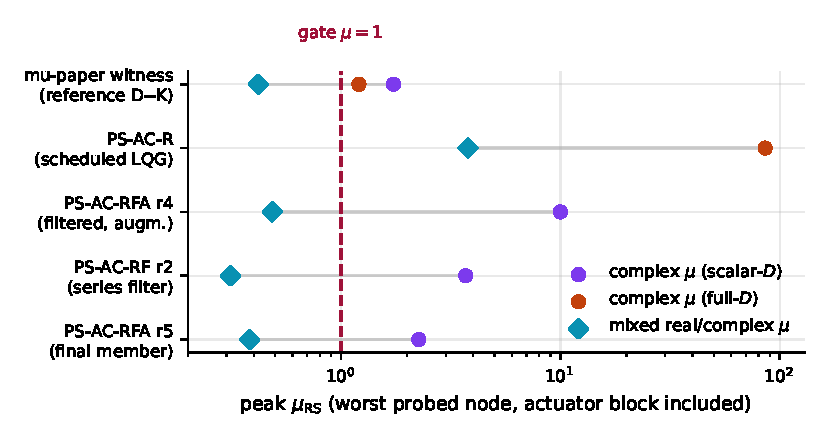
\includegraphics[width=.86\linewidth]{figs/fig_readings.pdf}
\caption{One gate, two prices.  Peak $\muRS$ (worst probed node,
actuator block included) under the complex readings used by the
benchmark's machinery and under the mixed real/complex reading.  Every
mixed value is a numerically verified upper bound.  The complex reading
overprices the parametrics by $4$--$8\times$ on gate-relevant
controllers and by $20\times$ on the scheduled-LQG barrier.}
\label{fig:readings}
\end{figure}

\begin{figure}[t]
\centering
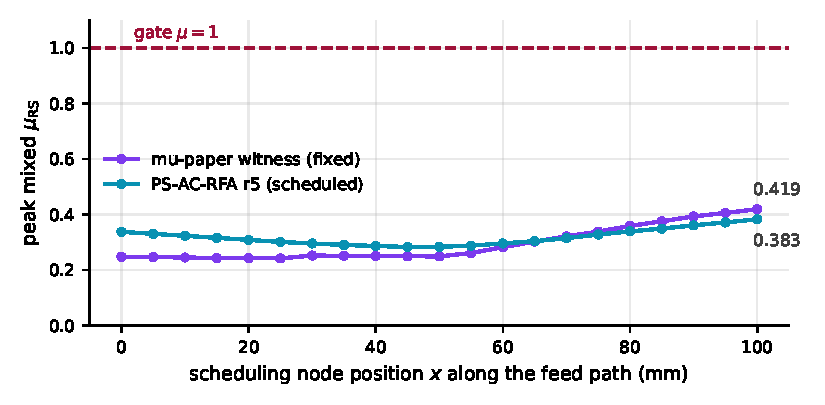
\includegraphics[width=.8\linewidth]{figs/fig_sweep21.pdf}
\caption{The full-domain gate: peak mixed $\muRS$ at each of the 21
scheduling nodes for the benchmark's fixed controller (witness) and the
scheduled member of Section~\ref{sec:member}.  Both curves clear the
gate at every node with margin $\ge 2.4\times$; the binding node is the
free end, where the removed-mass fraction acts most strongly.  The
complex reading on the same grid spans $1.63$--$1.73$ (witness) and
$2.11$--$2.27$ (member).}
\label{fig:sweep}
\end{figure}

\begin{enumerate}
\item \emph{The witness passes everywhere.}  The benchmark's own stored
controller, judged by its own complex machinery at $1.156$--$1.205$
(full-$D$) and $1.63$--$1.73$ (scalar-$D$), reads $0.242$--$0.419$
mixed across all 21 nodes---gate met at every node, worst at the free
end (1042\,Hz).
\item \emph{The scheduled-LQG barrier is real.}  The unfiltered
scheduled-LQG member reads $3.76$--$3.79$ mixed (complex: $85.8$): its
actuator-band violence is a genuine physical failure, not a reading
artifact.  Actuator-aware filtering is therefore necessary, not
cosmetic.
\item \emph{``Complex-fragile'' can be ``real-deep''.}  A series-filter
member whose complex reading collapsed ($2.9$--$3.7$) is among the
deepest gate-crossers in the mixed reading ($0.249$--$0.313$): its
fragility was entirely in the reading.
\end{enumerate}

For completeness, the complex-reading gate itself was closed
reproducibly before being re-read: a jitter-certified weight search
(perturbing frequency grids and weight corners by $\pm\varepsilon$)
shows the best \emph{reproducible} complex-reading optimum of the D--K
family at $1.728$, while apparently better runs at $1.400$ are lucky
draws whose jitter-certified values are $8.59$ and $4.08$.

\subsection{Scheduling the delayed pair is not a lever}

The cheapest scheduled attack on the gate--performance question keeps
the witness base and schedules only the delayed pair of the TDC law
with position, tracking the rank-one regenerative boundary
$a_4 D(x)^{\!\top} D(x)$ instead of freezing it at midspan (six
parameters, same count as $\mu$-TDC).  Under the full stage protocol
the result is a tie within bisection accuracy, a hair \emph{below} on
every axis: certified depth $0.4305$ vs $0.4364$\,mm, margin
$1.535$ vs $1.543$, nominal floor $0.6792$ vs $0.6821$\,mm, mean floor
$0.981$ vs $1.006$\,mm.  The hypothesis ``freezing the pair at midspan
loses something material'' is falsified by measurement.  Combined with
item~1 above, this yields the cleanest reading of the benchmark:
\emph{under the corrected pricing, the study's own $\mu$-TDC already
carries the gate and the performance floors simultaneously}; what
scheduling still owes is a floor improvement on a gate-crossing base.

\section{An actuator-aware scheduled member, and three structural
results}
\label{sec:member}

\subsection{The filter belongs inside the design model}

Because the barrier of item~2 is physical, the scheduled member is
synthesised with its actuator-protection filter (three notches at the
truncated modes $2787/3351/4122$\,Hz plus a second-order roll-off)
\emph{inside} the design model: an augmented LQR on the joint state
(filter; plate) at each scheduling node, with the observer estimating
the plate alone, driven by the exact filtered command.  Two structural
failures motivate this choice, both measured: the series
arrangement breaks certainty equivalence (its parametric performance
collapsed twice under pressure), and an ``observer-consistent''
shortcut that rewires the observer around the plain-plant LQR carries
an unstable internal observer--filter loop (closed-loop poles at
$+2\times10^{5}$\,1/s): separation does not survive lag in the command
path.

The augmented Riccati equation is numerically hostile---filter states
carry volt-sized signals and plate states metre-sized ones, eight
decades apart---and is solved in scaled coordinates (an exact diagonal
similarity; the gain is invariant, verified byte-identical where the
raw solve succeeds).

The final member (round 5) is an 8-parameter, order-14 controller
with fastest pole $5.0\times10^{4}$\,rad/s ($\approx 8$\,kHz),
$M_s = 1.675$, effort $151$\,V/N; its gate numbers appear in
Fig.~\ref{fig:sweep} (point $0.283$--$0.383$ over 21 nodes; worst
interpolation cell $0.320$), and its nominal position floor at the
reference speed is $0.419$\,mm across the five probe positions
($[0.42, 0.84, 0.72, 1.06, 0.53]$\,mm)---above the benchmark reference
depth of $0.3$\,mm.

\subsection{Three measured structural results}

\paragraph{(a) A $J$-ceiling of the filtered structure, with its named
challenger rejected.}  Three independent synthesis rounds under
different constraint sets converge to $J \approx -0.28$
(seeds: $-0.288/-0.281/-0.326$): the price of actuator-channel
robustness for this structure is $\approx 0.42$ of $J$ relative to the
unfiltered member ($+0.145$) that fails the gate at $3.8$.  The one
named candidate to break the ceiling---first-order phase-lead
compensation inside the design model (10 parameters)---was searched
under the identical protocol and rejected: best seed
$J = -0.339$, and the optimiser parks both lead parameters at their
lower bounds ($f_{\mathrm{lead}} = 424$\,Hz at bound 400;
$k = 1.56$ at bound 1.5), i.e.\ it tries to switch the lead off: phase
advance is bought with high-frequency gain that the actuator-band
constraint immediately bills.

\paragraph{(b) The baseline performance is mortgaged to unimplementable
poles.}  The stored scheduled-LQG member of the baseline study
($J = +0.145$) carries compensator poles at up to $8.8$\,MHz (family
range $1.4$--$8.8$\,MHz), originating from both the LQR and Kalman
sides.  Re-running its own synthesis inside realizability bounds
(gain ratio $\le 10^{9}$, poles $\le 2\pi\cdot20$\,kHz) lands at
$J = -0.482$ with two agreeing seeds.  The gap of $0.63$ in the shared
objective is the price of implementability for the scheduled-LQG
structure and re-prices every performance comparison built on the
stored gains.  The pathology has a certification-side twin, measured:
for an LQG member carrying ${\sim}2$\,MHz parasitic poles the
pointwise disc margin is huge ($0.05$) and a certificate is guaranteed
to exist by Proposition~\ref{prop:kyp}, yet no floating-point
construction we tried can exhibit one---the
${\sim}4{\times}10^{3}$ closed-loop dynamic range drives the Riccati
conditioning past float64 verification floors
(\texttt{mu\_real\_cmp.npz}, \texttt{adiab\_cmp.npz}).

\paragraph{(c) A realizable envelope-law member for certification.}
For the whole-pass certificate below we also carry \texttt{PS-AC-RI}:
the same envelope design law inside explicit realizability bounds
($J=-0.482$, $M_s = 1.82$, poles $\le 1.2\times10^{5}$\,rad/s,
5 parameters)---deliberately heavy damping and a tame realization.
Judged under the mixed reading it meets the gate as well, at
$\muRS = 0.688$--$0.690$ across the probed nodes (complex reading:
$15.6$), so the certification member of Section~\ref{sec:pass}
carries the gate and the whole-pass certificate simultaneously.

\section{The whole-pass certificate}
\label{sec:pass}

\subsection{Chain form: cells, jumps, dwell}

The repository's two delay certificates each miss what milling does:
the exact crossing test freezes the schedule (each point judged with
its own member, nothing certifies the traversal), and a common-$P$ LK
certificate prices arbitrarily fast variation the machine never uses.
The whole-pass certificate is built instead from the study's own
delay-independent LK form given an exponential rate: for cell $i$ with
frozen member and vertex family $(A, A_d)$,
\begin{equation}
V_i = x^{\!\top} P_i x + \int_{t-\tau}^{t} e^{2\alpha(s-t)}
      x(s)^{\!\top} Q_i\, x(s)\, ds, \qquad
\Phi_i = \begin{bmatrix} A^{\!\top}P_i + P_iA + 2\alpha P_i + Q_i &
P_iA_d \\ A_d^{\!\top}P_i & -e^{-2\alpha\tau} Q_i \end{bmatrix}
\prec 0 .
\label{eq:lk}
\end{equation}
This is the classical delay-independent LK form \cite{Gu2003} given an
exponential rate; feasibility at $(\alpha, \tau)$ covers every delay
$\tau' \le \tau$ (all faster spindle speeds).  At a cell switch the
state and history are continuous, so $V_{i+1} \le \mu\, V_i$ for every
history iff $P_{i+1} \preceq \mu P_i$ and $Q_{i+1} \preceq \mu Q_i$;
the recorded jump factor is the largest generalized eigenvalue over
the stored pairs.  Monotone traversal with dwell $h_k / v$ then gives
the certified traversal speed
\begin{equation}
\vcert = \min_k \; 2\alpha h_k / \ln \mu_k ,
\label{eq:vcert}
\end{equation}
to be compared with the actual feed speed: the certificate consumes
the known slowness of the schedule instead of paying common-$P$'s
price.  The two statements underlying the chain are the following
(proofs in Appendix~\ref{app:proofs}).

\begin{proposition}[delay cover]\label{prop:cover}
If $P, Q \succ 0$ satisfy $\Phi \prec 0$ in \eqref{eq:lk} for delay
$\tau$ and rate $\alpha \ge 0$, then the same pair certifies decay
rate $\alpha$ for every \emph{constant} delay $\tau' \in [0, \tau]$
(the tooth period is constant within a pass at fixed spindle speed;
shorter delays are faster speeds).
\end{proposition}

\begin{theorem}[finite-cell chain]\label{thm:chain}
Partition the pass into cells $I_k$ of length $h_k$ and let
$(P_k, Q_k) \succ 0$ satisfy \eqref{eq:lk} with rate $\alpha > 0$
uniformly over the closed convex model hull of cell $k$ (vertex family
plus a norm-$\varepsilon_k$ residual absorbed by the S-procedure of
Lemma~\ref{lem:sproc}).  For $X, Y \succ 0$ write
$\lambda_{\max}(X, Y) = \min\{\mu : X \preceq \mu Y\}$, the largest
generalized eigenvalue of the pencil $(X, Y)$; let
$\mu_k = \max\{\lambda_{\max}(P_{k+1}, P_k),\,
\lambda_{\max}(Q_{k+1}, Q_k)\}$ denote the boundary jump factors, and
let the schedule traverse the cells monotonically at speed $v$.  If
$\ln \mu_k \le 2\alpha h_k / v$ at every boundary, then for every
parameter path in the tube and every delay $\tau' \le \tau$ the closed
loop is exponentially stable over the whole pass, with
\[
V(t) \;\le\; \exp\Big({-2\alpha (t - t_0)} +
\textstyle\sum_{\text{switches}\le t} \ln \mu_k\Big)\, V(t_0);
\]
equivalently, every traversal speed $v \le \vcert$ of
\eqref{eq:vcert} is certified.
\end{theorem}

\subsection{Pointwise equivalence, and an empirical obstruction law}

Cell-wise SDP solves of \eqref{eq:lk} refuse on this plant even for
near-nominal tubes.  A diagnosis ladder isolates why, in two steps.

\emph{First, the pointwise tests agree.}  For rank-one delayed coupling
$A_d = b\,c^{\!\top}$ (verified: $\sigma_2/\sigma_1 = 1.4\times
10^{-16}$ for the LQG-type members), the exact crossing measure
$\sup_\omega \rho\!\big((j\omega I - A)^{-1} A_d\big)$ \emph{is} the
delay-disc measure $\|G\|_\infty$ of the scalar channel
$G(s) = c^{\!\top}(sI - A)^{-1} b$: no phase is lost between the
crossing test and the DI premise.  More is true, by an elementary
frequency-domain argument:

\begin{proposition}[rank-one KYP equivalence]\label{prop:kyp}
Let $A$ be Hurwitz and $A_d = b c^{\!\top}$.
(a)~If $P, Q \succ 0$ satisfy $\Phi \prec 0$ in \eqref{eq:lk} for some
$\alpha \ge 0$, then $\|G\|_\infty < 1$.
(b)~Conversely, if $\|G\|_\infty < 1$ then, at $\alpha = 0$, the
aligned pair $Q = c\,c^{\!\top} + \delta I$ (small $\delta > 0$) with
$P$ the stabilising solution of a strict bounded-real Riccati equation
satisfies $\Phi \prec 0$; by continuity the same holds for all
sufficiently small $\alpha > 0$.
(Proof in Appendix~\ref{app:proofs}.)
\end{proposition}

Measured on a refused
cell: all 32 vertices pass pointwise ($\|G\|_\infty \in
[0.040, 0.541]$), yet the SDP reports infeasible even for a
\emph{single} vertex with a $25\times$ margin.  Rebuilding that
certificate without any optimiser (below) yields a verified functional
with margin $-5.8\times10^{-7}$: \emph{the recorded single-vertex SDP
refusals are solver failures}, and the verification-gated design of the
pipeline (``an inaccurate solve can only produce a certificate that
verifies, or none'') correctly reported ``no certificate'' while
inviting the wrong mechanism story.

\emph{Second, the cell refusals are structural, with a quantitative
empirical law.}  We state this deliberately as a measured observation
rather than a theorem: the anisotropy of any certifying storage on
this plant (eigenvalue range set by the $\sim\!10^4$ frequency ratio
of the retained modes) makes a sharp analytic necessity bound
unwieldy, while the measurement is unambiguous.  The vertex spread
inside any practical cell rotates the
razor-thin modal eigendirections by many half-power linewidths
($\zeta\omega$): an 8-vertex $\theta$-corner family spreads
$\|\Delta A\| = 4\times10^{-3}$ against a linewidth of
$2\times10^{-3}$ (scaled), and the position axis alone contributes
$\approx 700$ linewidths per twentieth of the span.  A single quadratic
storage across eigendirections rotated by more than a linewidth cannot
exist; the feasible cell diameter scales with $\zeta$, not with the
tube.  This replaces our earlier, incorrect naming of the mechanism
(``constant scales vs.\ rank-one coupling''), a correction kept on the
record.

\subsection{Solver-free point certificates}

The cell certificate is therefore rebuilt at a point (and later chained
densely).  Fix $Q = w\,\overline{A_d^{\!\top} A_d} + q_0 s_Q I$ first
(aligned with the delayed output directions); by the Schur complement
on \eqref{eq:lk} the coupling term is then a known Riccati channel, and
\begin{equation}
A_c^{\!\top} P + P A_c + 2\alpha P
+ P \Big[\tfrac{s}{e^{-2\alpha\tau}}\,
\overline{A_d Q^{-1} A_d^{\!\top}} + \kappa\, \Sigma_{\mathrm{in}}
\Big] P + (1{+}m) Q + \tfrac{1}{\kappa}\,\Sigma_{\mathrm{out}}
+ m\, s_Q I = 0
\label{eq:ric}
\end{equation}
is solved on the stable invariant subspace of its Hamiltonian
(balanced by the exact substitution $P = \theta \tilde P$,
$\theta^2 = \mathrm{tr}\,C^{\!\top}C / \mathrm{tr}\,BB^{\!\top}$),
where the $\kappa$-terms absorb vertex spread by a directional Young
inequality on the thin-SVD factors of $\Delta A$.  \emph{Every}
candidate is judged solely by the numerical verifier (eigenvalue tests
of $\Phi$, $P$, $Q$); nothing rests on the construction.  A point
certificate costs milliseconds; there is no optimiser in the loop.

\subsection{The adiabatic (thin-cell) limit, measured to completion}

With point certificates $P(x_k), Q(x_k)$ every $h$ along the pass and
scale-balanced neighbour costs
$\ln\mu_k = \tfrac12 \ln\big(\lambda_{\max}(P_{k+1}, P_k)\,
\lambda_{\max}(P_k, P_{k+1})\big)$ (and likewise $Q$),
\eqref{eq:vcert} becomes, as $h \to 0$,
$\vcert \to \min_x 2\alpha / \rho(x)$ with rotation density
$\rho = d \ln\mu / dx$.  Constant-in-time uncertainties are
\emph{sliced}---$a_4$ and $\zeta$ do not evolve during a pass, so each
realization keeps one chain and the guarantee is the minimum over
slices---while the evolving quantities ($x$, and the removal pair
$\eta, \xi$) are chained.  Four measurement campaigns close the limit:

\begin{figure}[t]
\centering
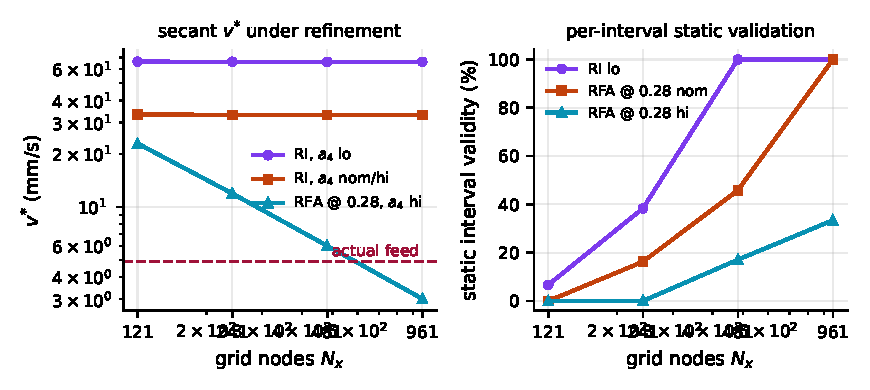
\includegraphics[width=.98\linewidth]{figs/fig_refine.pdf}
\caption{Grid refinement as an honesty instrument.  Left: secant
$v^{*}$ under refinement---the realizable member converges on every
slice, while the filtered member's $a_4$-hi slice at $\ap=0.28$\,mm
\emph{diverges} ($22.9 \to 3.0$\,mm/s, below the actual feed): the
coarse-grid certificate was over-optimistic and is corrected.  Right:
fraction of intervals whose stored functional statically certifies
their left/mid/right models; $100\%$ means a fully verified finite
chain with no limit argument left open.}
\label{fig:refine}
\end{figure}

\begin{figure}[t]
\centering
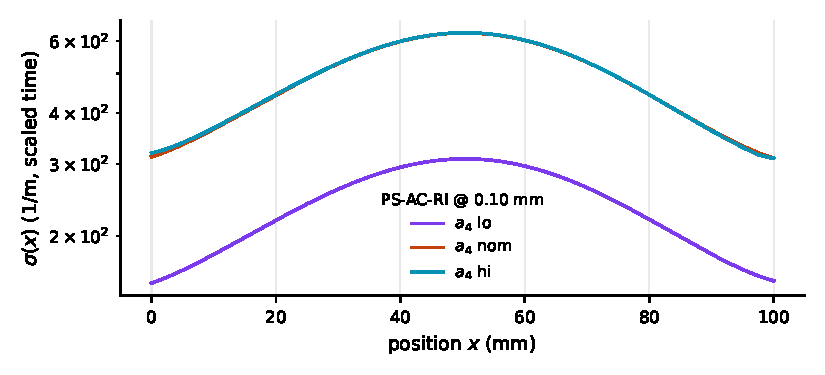
\includegraphics[width=.8\linewidth]{figs/fig_sigma.pdf}
\caption{The differential rotation cost $\sigma(x)$ of the
frozen-parameter Riccati chains for the realizable member (three
$a_4$ slices, $h/2$ grid).  $\sigma$ is converged under grid halving
(ratios $0.96$--$0.98$) and the pointwise LMI margins are re-verified
at $100\%$ of the nodes: every hypothesis of
Theorem~\ref{thm:diff} is measured.}
\label{fig:sigma}
\end{figure}

\paragraph{(i) Slices and rate optimisation.}
Across all nine $a_4\times\zeta$ slices, with the decay rate $\alpha$
ladder-optimised per slice, the realizable member at $\ap = 0.10$\,mm
certifies at $\vcert = 82.7$\,mm/s (worst slice, converged under
refinement).  Against the actual feed of $4.90$\,mm/s this is a rate
margin $\vcert / v_{\mathrm{feed}} \approx 16.9$: the physical
schedule evolves $16.9\times$ more slowly than the fastest evolution
the certificate tolerates.  We stress the interpretation: this is a
robustness margin on the schedule rate, \emph{not} a claim that
material removal could be increased $16.9$-fold.  The $\zeta$-slice rows
coincide; a wiring check confirms $\zeta$ reaches the model
($\|A(1.2)-A(0.8)\| = 2.2\times10^{-3}$), so this is genuine
certificate insensitivity to $\pm20\%$ damping.

\paragraph{(ii) Static validation of finite chains.}
Upgrading the $O(h^2)$ residual argument to measurement: an interval is
\emph{statically valid} if its stored functional certifies the models
at its left, mid and right samples.  The realizable member's $a_4$-lo
slice reaches $100\%$ validity at $h = 0.104$\,mm
(Fig.~\ref{fig:refine}, right)---a fully verified finite chain.  The
nom/hi slices would need $h \sim 10^{-8}$\,m (margin/$\rho$) and stand
instead on the differential reading below.

\paragraph{(iii) A correction forced by refinement.}
The filtered member's full-box certificate at $\ap = 0.28$\,mm does
not survive refinement: its $a_4$-hi slice diverges
($v^{*}: 22.9 \to 3.0$\,mm/s $<$ feed as $N_x: 121 \to 961$), with
$\rho$ localising into a spike---the depth sits on the member's exact
crossing edge ($\ap^{\infty} = 0.2841$\,mm).  The full-box
\emph{statically validated} depth is $\ap = 0.15$\,mm
($100\%$ validity at $h = 0.104$\,mm, $v^{*} = 24.7$\,mm/s,
$5.0\times$ feed).  The $\rho$-spike divergence doubles as a
diagnostic for near-marginal corners that coarse grids flatter.

\paragraph{(iv) The live removal tube.}
Rotation densities along the removal axes are measured directly
($\rho_\eta \approx 645$ for the realizable member---removal motion
costs as much as position motion---and $\rho_\xi \approx 1.9$), giving
the composite path bound
$v^{*}_{\mathrm{path}} = \min_x 2\alpha / (\rho_x + \rho_\eta\,
\Delta\eta / \ell + \rho_\xi / \ell)$: with the entire admissible
removal in a single pass (worst case), $17.8$\,mm/s---still
$3.6\times$ the actual feed.

\subsection{The differential theorem, hypotheses measured}

\begin{theorem}[differential adiabatic chain]\label{thm:diff}
Let the schedule follow the pass at speed $v$ and, on each regime
interval, let $x \mapsto (P(x), Q(x))$ be a $C^1$ field of positive
definite matrices satisfying the pointwise LMI \eqref{eq:lk}, for the
slice model $(A(x), A_d(x))$, with rate $\alpha$ (in our
construction: the frozen-parameter Riccati field of \eqref{eq:ric},
which is real-analytic wherever the Hamiltonian retains its dichotomy
\cite{Lancaster1995}).  The functional evaluates both matrices at the
\emph{current} schedule point,
$V(t) = x^{\!\top} P(x(t))\, x + \int_{t-\tau}^{t} e^{2\alpha(s-t)}
x(s)^{\!\top} Q(x(t))\, x(s)\, ds$.  Define
$\sigma(x) = \max\big(\|P^{-1/2}P'P^{-1/2}\|_2,\,
\|Q^{-1/2}Q'Q^{-1/2}\|_2\big)$, and let regime boundaries carry jump
factors $\mu_b$ as in Theorem~\ref{thm:chain}.  Then $V$ of
\eqref{eq:lk} satisfies
$\dot V \le (-2\alpha + v\,\sigma(x))\,V$ inside regimes and
$V^{+} \le \mu_b V$ at boundaries; consequently the whole pass is
exponentially stable whenever
$v < \min_x 2\alpha/\sigma(x)$ and the dwell rule holds at each
boundary; by Proposition~\ref{prop:cover} the statement again covers
every constant delay $\tau' \le \tau$.
(Proof in Appendix~\ref{app:proofs}.)
\end{theorem}

Measured on this plant (Fig.~\ref{fig:sigma}): the winner-parameter
census returns a \emph{single} frozen construction per slice across
the whole domain (61/61 nodes---no regimes, no jumps); pointwise
margins verify at $100.0\%$ of the fine-grid nodes on every slice of
both members; and $\sigma$ is converged under $h \to h/2$ (ratios
$0.958$--$0.984$).  The theorem-grade speeds,
$v^{*}_{\mathrm{diff}} = 79.9$\,mm/s (realizable member,
$\ap=0.10$\,mm, worst slice) and $23.6$\,mm/s (filtered member,
$\ap = 0.15$\,mm), confirm the secant estimates within $\approx3\%$.

\subsection{Scope: delay-exploiting members}

TDC-type members \emph{use} the delay by design (their delayed pair is
part of the law, and their delayed coupling is genuinely rank-two:
$\sigma_2/\sigma_1 = 0.56$), so ``stable for every
$\tau' \le \tau$'' is not their contract; they rightly fail the
pointwise disc at 46--100 of 121 nodes.  Their whole-pass statement
belongs to the exact-crossing instrument; the certificate developed
here covers the delay-agnostic (LQG-type) members.

\section{Summary of certified results}

\begin{table}[t]
\centering\small
\caption{Final certified numbers (actual feed $4.90$\,mm/s; every row
recomputable from stored matrices).  Ratios $\vcert /
v_{\mathrm{feed}}$ are robustness margins on the schedule rate---how
much faster the process state could evolve with the certificate still
valid---not productivity figures.}
\label{tab:final}
\setlength{\tabcolsep}{4pt}
\begin{tabular}{@{}p{4.4cm}p{4.0cm}p{1.9cm}p{4.8cm}@{}}
\toprule
Quantity & Value & Rate margin & Basis \\
\midrule
Gate, witness, 21/21 nodes & $\muRS \le 0.419$ & $\ge 2.4\times$ &
mixed $\mu$, verified scales \\
Gate + cell, scheduled member & $0.283$--$0.383$; cell $0.320$ &
$\ge 2.6\times$ & idem \\
Whole pass, realizable, $\ap{=}0.10$ & $\vcert = 82.7$ ($79.9$ diff.)
\,mm/s & $16\times$ & 9 slices, $\alpha$-opt., converged \\
\quad with live removal schedule & $17.8$\,mm/s & $3.6\times$ &
worst single-pass $\Delta\eta$ \\
Whole pass, filtered, full box & $\ap = 0.15$\,mm, $v^{*}{=}24.7$
($23.6$) & $5\times$ & static validity $100\%$ at $h{=}0.104$\,mm \\
Performance ceiling (filtered) & $J = -0.281$ & --- & 3 rounds;
lead probe $-0.339$ rejected \\
Realizability price (sched.\ LQG) & $\Delta J = 0.63$ & --- &
$+0.145$ (8.8\,MHz poles) vs $-0.482$ \\
\bottomrule
\end{tabular}
\end{table}

Table~\ref{tab:final} collects the headline numbers; they are the
\emph{demonstration} of Theorems~\ref{thm:chain}--\ref{thm:diff} on
a validated plant, not the contribution itself.

\subsection*{Baseline comparison of certification routes}

Table~\ref{tab:baseline} makes the value case directly: the same
plant and the same controllers, judged by the four certification
routes a practitioner could take.  The frozen conservative-set route
(the benchmark's practice) refuses the gate outright under its
complex reading; frozen-point analysis under the corrected reading
meets the gate at every node but says nothing about any $v > 0$
between the nodes; and the classical cell-wise common-storage route
is \emph{measured} here on a cell-size ladder
(\texttt{baseline\_cmp.npz}; nominal slice, three samples per cell,
no residual---an upper bound on its feasibility): it is infeasible at
every practical granularity, becoming feasible only at
$h \le 0.1$\,mm for the realizable member ($1000$ cells over the
pass; sample spread $6\times10^{-3}$, i.e.\ $3$--$6$ linewidths---an
independent probe of the empirical $\zeta$-scaling law of
Section~\ref{sec:pass}) and $h \le 2.5$\,mm for the more heavily
damped filtered member.  Moreover, at the granularity where per-cell
common storage finally exists, it still yields no traversal statement
without jump factors and a dwell rule---that is, without
Theorem~\ref{thm:chain}: the classical baseline collapses into the
present method exactly where it starts to work.

\begin{table}[t]
\centering\small
\caption{Baseline comparison: what each certification route delivers
on the same plant and controllers.  ``---'' = the route produces no
statement of that kind.}
\label{tab:baseline}
\begin{tabular}{@{}p{4.6cm}p{4.2cm}p{5.2cm}@{}}
\toprule
Certification route & Gate verdict & Whole-pass statement \\
\midrule
Frozen conservative set, complex $\mu$ (benchmark practice) &
refused: $1.156$--$1.205$ (witness, its own judge); $2.1$--$2.3$
(scheduled member) & --- (no certificate at any speed) \\
Frozen-point mixed $\mu$, 21 nodes &
met: $0.242$--$0.419$ / $0.283$--$0.383$ &
--- (no statement for any $v > 0$) \\
Common quadratic LK storage (classical cell-wise LMI) &
n/a &
infeasible for $1$--$500$ cells (realizable member) and $1$--$20$
cells (filtered); feasible only at $h \le 0.1$ / $2.5$\,mm, and even
then requires Theorem~\ref{thm:chain} to stitch cells \\
Point-certificate chain + differential limit (this work) &
met, full 21-node domain &
$\vcert = 79.9$--$82.7$\,mm/s (full box; rate margin
${\approx}16\times$); $17.8$\,mm/s live tube; $23.6$--$24.7$\,mm/s
(filtered member, full box, $\ap = 0.15$\,mm) \\
\bottomrule
\end{tabular}
\end{table}

\subsection*{Head-to-head with the benchmark controller}

The controller comparison of this paper is deliberately confined to
the one comparison that is beyond fairness dispute: the benchmark's
own published controller, on the benchmark's own plant, judged by the
shared protocol (Table~\ref{tab:head2head}).  The comparison is
respectful by measurement: under the corrected pricing, $\mu$-TDC
already carries the gate and the depth floors simultaneously
(Section~\ref{sec:readings}), and scheduling its delayed pair buys
nothing (the tie of Section~\ref{sec:readings})---within its own
class the benchmark controller is close to optimal.  What the
scheduled members add over it is orthogonal: a whole-pass certificate
its delay-exploiting structure cannot receive under the
delay-independent contract (its own whole-pass evidence remains the
frozen-point crossing sweep, full-box peak $0.613$ at the reference
depth), a realizable member that carries gate and pass certificate
together, and---for the filtered member---scenario recovery
$3.0\times$ faster at $0.45\times$ the control energy and
$0.71\times$ the voltage peak.  The price is equally measured and
stated: lower certified depth floors ($0.284$ vs $0.436$\,mm
crossing; $0.419$ vs $0.682$\,mm nominal floor).  This is a measured
frontier between depth headroom and certified traversal with faster,
cheaper recovery---not a domination claim.
One marginality is stated rather than hidden: the realizable
member's worst-position nominal limit ($0.299$\,mm) sits essentially
at the reference depth ($0.3$\,mm), so at that condition it operates
with the thinnest depth margin of the three (its time response there
remains quiet, $4.1\,\mu$m peak, Fig.~\ref{fig:timeresp}).
The lobe-first round below narrows the depth side of this frontier
within the same protocol.

\begin{table}[t]
\centering\small
\setlength{\tabcolsep}{5pt}
\caption{Head-to-head with the benchmark controller under the shared
protocol.  Gate = peak mixed $\muRS$ over the probed nodes (complex
reading in parentheses).  S1 recovery ratios are relative to
$\mu$-TDC ($=1$).  Sources: \texttt{stage3\_controllers.pkl},
\texttt{stage56.pkl}, \texttt{stage78.pkl},
\texttt{mu\_real*.npz}, \texttt{adiab\_*.npz}.}
\label{tab:head2head}
\begin{tabular}{@{}p{4.6cm}p{3.4cm}p{3.6cm}p{3.2cm}@{}}
\toprule
 & $\mu$-TDC (benchmark) & PS-AC-RFA r5 & PS-AC-RI \\
\midrule
parameters / order & 6 / 12 & 8 / 14 & 5 / 6 \\
$J$ (shared objective) & $-0.025$ & $-0.281$ & $-0.482$ \\
$M_s$ / effort (V/N) & $2.00$ / $152$ & $1.68$ / $151$ & $1.82$ /
$109$ \\
gate, mixed $\muRS$ & $0.242$--$0.419$ ($1.16$--$1.21$) &
$0.283$--$0.383$; cell $0.320$ ($2.1$--$2.3$) & $0.688$--$0.690$
($15.6$) \\
crossing $\ap^{\infty}$ / $\delta_{\max}$ & $0.436$\,mm / $1.543$ &
$0.284$\,mm / $0.918$ & --- \\
nominal floor / mean (mm) & $0.682$ / $1.006$ & $0.419$ / $0.712$ &
$0.299$ / $0.474$ \\
recovery: time / energy / peak & $1$ / $1$ / $1$ &
$0.33$ / $0.45$ / $0.71$ & $0.21$ / $0.12$ / $0.64$ \\
whole-pass certificate & out of DI contract (TDC); frozen-point
crossing, peak $0.613$ & $\vcert = 23.6$--$24.7$\,mm/s, full box,
$\ap = 0.15$\,mm & $\vcert = 79.9$--$82.7$\,mm/s full box;
$17.8$ live tube \\
\bottomrule
\end{tabular}
\end{table}

\subsection*{Stability lobes and time-domain response}

Figures~\ref{fig:lobes} and~\ref{fig:timeresp} present the two views
the machining community reads first, computed with the repository's
own validated machinery (the Floquet bisection on the five-mode truth
model; the Newmark time integration of the scenario protocol).  The
lobe chart is the \emph{minimum over the tool-path positions}
$\{0, L/2, L\}$---the machine-usable curve for a part whose dynamics
change along the feed path---and it is also where the shared protocol
showed its one measured blind spot: the objective $J$ probes the
design speed only, so the $J$-protocol members were never asked about
the rest of the band, and their lobe floors over $3600$--$7200$\,rpm
($0.340$\,mm filtered, $0.232$\,mm realizable) sit well under the
benchmark's $0.474$\,mm.  The lobe-first round below closes most of
that gap within the same constraints; the figures carry its
gate-passing filtered champion PS-AC-RFA-L ($0.439$--$0.729$\,mm)
next to $\mu$-TDC ($0.474$--$0.802$\,mm), the realizable member
($0.232$--$0.656$\,mm), the family's delay-exploiting member
($0.583$--$1.349$\,mm, dashed---its classification is measured
below), and the open loop ($0.039$\,mm worst)---all lifted from the
open-loop floor by roughly an order of magnitude.  In the time domain
at the reference condition the open loop diverges within $0.089$\,s,
while the members hold the response at $2$--$4\,\mu$m with peak
actuation of $16$--$37$\,V---far inside the $450$\,V authority.

\begin{figure}[t]
\centering
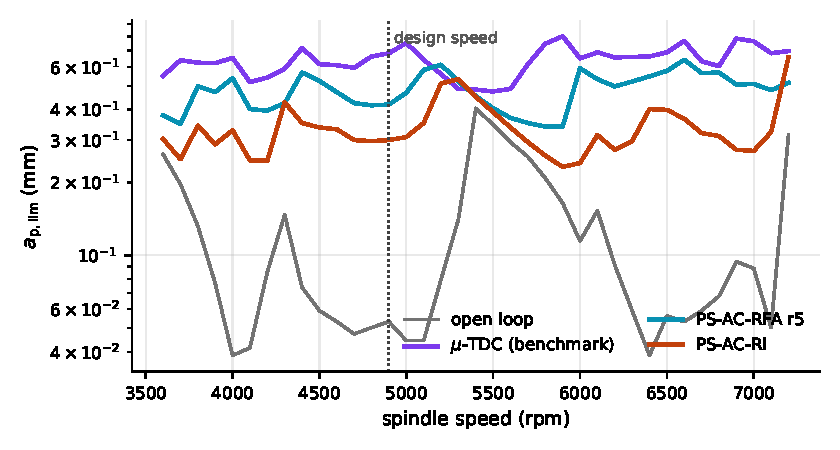
\includegraphics[width=.8\linewidth]{figs/fig_lobes.pdf}
\caption{Stability lobes: critical depth of cut vs.\ spindle speed,
minimum over the tool-path positions $\{0, L/2, L\}$ (five-mode truth
model, Floquet $m = 120$, bisection to $5\,\mu$m).  PS-AC-RFA-L is
the lobe-first champion of Section~\ref{sec:lobefirst}; the dashed
curve is the family's delay-exploiting member (out of the DI contract
and the gate, as marked in Table~\ref{tab:lobefirst}).  The dotted
line marks the design speed.  Sources: \texttt{lobes\_l2.npz},
\texttt{lobes\_tdcj.npz}.}
\label{fig:lobes}
\end{figure}

\begin{figure}[t]
\centering
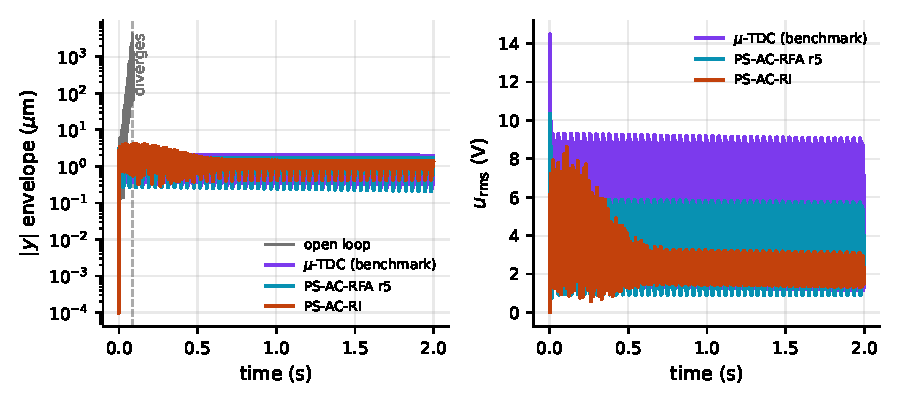
\includegraphics[width=.95\linewidth]{figs/fig_timeresp.pdf}
\caption{Time response at the reference condition ($4900$\,rpm,
$\ap = 0.3$\,mm, moving cut, $2$\,s window).  Left: displacement
envelope at the sensor (log scale)---the open loop diverges at
$t = 0.089$\,s (dashed vertical marker); the members hold a
$2$--$4\,\mu$m peak and settle near or below $1\,\mu$m.  Right: rms
actuation voltage of the members.
Sources: \texttt{timeresp.npz}, \texttt{timeresp\_l.npz},
\texttt{timeresp\_tdcj.npz}.}
\label{fig:timeresp}
\end{figure}

\subsection*{A lobe-first design round}
\label{sec:lobefirst}

The deficit above is a property of the design pressure, not of the
scheduled structure, and it is treated the way every other gap in
this study was treated: measure the binding mechanism, change one
declared thing at a time, and let pre-declared bars judge the result
at full resolution (Floquet $m = 120$, $37$ speeds, min over
positions).  The bars, declared before the first search: L1, beat the
incumbent's floor; L2, beat the benchmark's $0.474$\,mm; L3, hold the
shared constraints---and the standing gate G1 disqualifies any winner
it rejects.

\emph{Round 1 (objective).}  The objective is replaced by the
lobe-floor functional---the same Floquet-margin functional as $J$,
extended over a nine-speed grid spanning the band at probe depths
$(0.5, 0.7, 0.9)$\,mm---with each swarm warm-started at its stored
$J$-protocol winner; structure, box, screens, optimiser and seeds are
untouched.  The filtered floor moves $0.340 \to 0.407$\,mm, the
realizable floor $0.232 \to 0.238$\,mm, and the binding pressures are
then \emph{measured}: the filtered winner stands at its self-imposed
corner-envelope bar (corner $M_s = 1.935$ of $2.0$) with both shared
constraints slack, while the realizable winner stands at its
search-box walls (gain ratio $8.999$ of $9$; poles
$1.246\times10^{5}$ of the $1.257\times10^{5}$\,rad/s cap) with
corner $M_s$ only $1.09$.

\emph{Round 2 (parity and walls).}  The benchmark controller itself
measures corner $M_s = 2.119$ on the same eight physics
corners---the corner bar imposed on our own member was stricter than
what the benchmark achieves.  Setting the member's corner bar to the
benchmark's own measured value (the shared nominal bar
$M_s \le 2.0$ is untouched) lifts the filtered floor to $0.439$\,mm,
and the shared constraint itself now binds exactly
($M_s = 1.999$)---the same bar the benchmark sits at ($2.00$).  A
ten-parameter phase-lead arm under identical pressures measures
\emph{worse} ($0.302$\,mm) and is recorded as a negative result.
Widening the realizable box in gain and ratio only (the certificate's
pole cap unchanged) lifts that class's floor to $0.314$\,mm and even
produces a reference-depth path certificate ($9.5$\,mm/s at
$\ap = 0.30$\,mm)---but the mixed gate rejects the winner
($\muRS = 1.21$--$1.23$ at every probed node): the realizable box is
thereby measured to be \emph{load-bearing for the gate}, not an
arbitrary restriction, and the paper's realizable member remains
PS-AC-RI.

\emph{Round 3 (ceiling).}  A polish at the judge's own resolution
($m = 120$) on exactly the six binding speeds, three independent
seeds, moves the filtered floor by less than $0.001$\,mm.  At equal
robustness bars on both sides, $0.439$ against $0.474$\,mm
($7.4\%$, with $31$ of $37$ speeds at or above the benchmark's
floor) is therefore the measured price of the delay-independent,
whole-pass-certifiable structure on this plant---the depth side of
the Table~\ref{tab:head2head} frontier, narrowed from $28\%$ and
quantified at its saturation.

Table~\ref{tab:lobefirst} carries the champion's full battery.  Its
gate record is complete at the same standard as the witness and the
r5 member: mixed $\muRS = 0.330$--$0.450$ over \emph{all} 21
scheduling nodes (worst at the free end), G1(real) met everywhere.
It improves the shared objective it was not optimised for
($J = -0.166$ vs $-0.281$), raises the nominal floor to $0.539$\,mm,
and keeps the $3.0\times$ faster scenario recovery (at $0.70\times$
the energy).  Its whole-pass certificate at $\ap = 0.15$\,mm, taken
through the incumbents' own per-slice $\alpha$ ladder with every
slice's static interval validation at $100\%$, reads
$\vcert = 246.6$\,mm/s over the nine $(a_4, \zeta)$ slices---a
$50\times$ rate margin against the actual feed, converged under grid
refinement, and \emph{ten times} the incumbent member's
$23.6$--$24.7$\,mm/s: the lobe-first push strengthened the
certificate rather than spending it.  The binding slice ($a_4$ hi,
$\alpha = 50$\,s$^{-1}$) reaches full static validity exactly at
$h = 0.104$\,mm---the same cell size the empirical $\zeta$-law fixed
for this class in Section~\ref{sec:pass}, reappearing here as the
validity scale of the point chain.

The remaining corner of the frontier is then measured rather than
conjectured.  The family's own delay-exploiting member
PS-TDC-J---the scheduled base with the grafted delayed pair, six
parameters as $\mu$-TDC, designed under the \emph{unchanged} shared
protocol---already carries a lobe floor of $0.583$\,mm: above the
benchmark's floor at all $37$ speeds, above the benchmark's own curve
pointwise at $31$ of $37$, with a nominal floor of $0.907$\,mm
($+33\%$ over $\mu$-TDC) and scenario settling $14\times$ faster
($T_s = 6.3$\,ms) at $0.79\times$ the energy ($1.48\times$ the
voltage peak, still far inside authority).  Its classification is
equally measured: it is out of the delay-independent contract by
design, and its unfiltered high-gain base fails the mixed gate
outright ($\muRS = 3.46$--$3.48$ at the probed nodes)---exactly the
exposure the gate exists to police.  Scheduling the delayed pair on
the witness base instead extends the tie of
Section~\ref{sec:readings} to the lobe axis (floor $0.472$ vs
$0.474$\,mm, pointwise above at only $16$ of $37$ speeds).  The
frontier is thereby priced in full on one plant under one protocol:
giving up the whole-pass certificate buys the step from $0.439$ to
$0.474$\,mm, and giving up the robustness gate as well buys the step
to $0.583$\,mm---each guarantee has a measured depth cost, and each
member of the family occupies exactly one declared corner
(Fig.~\ref{fig:lobes}, dashed curve; Table~\ref{tab:lobefirst}).

\begin{table}[t]
\centering\footnotesize
\setlength{\tabcolsep}{4pt}
\caption{The lobe-first round and the priced frontier.  Lobe rows are
full-resolution verdicts (Floquet $m = 120$, $3600$--$7200$\,rpm, min
over the tool-path positions); gate and recovery by the standing
machinery, each recovery ratio within one measurement batch.
PS-TDC-J is the family's delay-exploiting member under the unchanged
shared protocol.  Sources: \texttt{lobes\_l2.npz},
\texttt{lobes\_tdcj.npz}, \texttt{mu\_real\_l.npz},
\texttt{mu\_real\_tdcj.npz}, \texttt{s1\_l.npz},
\texttt{s1\_fresh.npz}, \texttt{s1\_tdcj.npz}, \texttt{cert\_l.npz}.}
\label{tab:lobefirst}
\begin{tabular}{@{}p{3.2cm}p{2.7cm}p{2.9cm}p{2.9cm}p{3.0cm}@{}}
\toprule
 & $\mu$-TDC (benchmark) & PS-AC-RFA r5 & PS-AC-RFA-L & PS-TDC-J
(delay-expl.) \\
\midrule
lobe floor, $3600$--$7200$\,rpm & $0.474$\,mm & $0.340$\,mm &
$0.439$\,mm & $0.583$\,mm \\
speeds at/above $0.474$\,mm & $37/37$ & $20/37$ & $31/37$ &
$37/37$ \\
nominal floor / mean (mm) & $0.682$ / $1.006$ & $0.419$ / $0.712$ &
$0.539$ / $0.886$ & $0.907$ / $1.373$ \\
gate, mixed $\muRS$ (nodes) & $0.242$--$0.419$ & $0.283$--$0.383$ &
$0.330$--$0.450$ ($21/21$) & $3.46$--$3.48$ (not met) \\
$M_s$ / effort (V/N) & $2.00$ / $152$ & $1.68$ / $151$ & $2.00$ /
$160$ & $1.98$ / $272$ \\
$J$ (shared objective) & $-0.025$ & $-0.281$ & $-0.166$ &
$+0.156$ \\
recovery: time / energy / peak & $1$ / $1$ / $1$ & $0.33$ / $0.45$ /
$0.71$ & $0.33$ / $0.70$ / $0.98$ & $0.07$ / $0.79$ / $1.48$ \\
whole-pass certificate & out of DI contract & $23.6$--$24.7$\,mm/s
(\mbox{$\alpha$-opt}), $\ap = 0.15$\,mm & $246.6$\,mm/s
(\mbox{$\alpha$-opt}, $100\%$ static validity), $\ap = 0.15$\,mm &
out of DI contract (as the benchmark) \\
\bottomrule
\end{tabular}
\end{table}

Under the corrected
pricing the spatio-temporal variation is no longer an adversary to be
over-insured against: it is measured, scheduled, sliced where
constant, chained where moving, and the guarantee runs over the
entire operating domain with an explicit rate margin against the
actual feed.

\clearpage
\section{Limitations and outlook}

We state the boundaries of the claims as measured.  (1)~All results are
model-based certifications on the (experimentally validated) benchmark
plant of \cite{Du2024}; no new experiments are reported.  (2)~The
nom/hi slices of the realizable member rest on the differential
reading of Theorem~\ref{thm:diff}; their static cell validation is
physically out of reach ($h \sim 10^{-8}$\,m).  (3)~The
$\eta/\xi$ tube enters the headline slice numbers frozen at midspan
and enters the path bound through measured densities under a
single-pass worst case; a fully coupled $(x, \eta, \xi)$ chain is
mechanical with the same tooling.  (4)~The decay rate $\alpha$ is
grid-optimised, not continuously optimised.  (5)~The performance
objective $J$ is the benchmark's Floquet-margin protocol; other
objectives may re-order members but not the certificates.
(6)~Deep-cut corners near a member's exact crossing edge are
intrinsically hostile to the DI premise (the measured $\rho$-spike);
certification there should be attempted at the exact delay only.
(7)~The lobe-first champion's crossing pair
($\ap^{\infty}, \delta_{\max}$) has not been re-measured; the
frozen-speed lobe verdicts of Table~\ref{tab:lobefirst} are the
sharper statement of the same axis.  Its certificate is
$\alpha$-optimised with full static interval validation
(\texttt{cert\_l2.npz}); the certified depth itself remains
$0.15$\,mm, not the reference depth.

\paragraph{Significance.}
Beyond the benchmark, the paper argues for three transferable
practices.  First, robustness gates on lightly damped structures
should be reported under the mixed real/complex reading: on this
plant the reading, not the physics, decided the gate, and the same
inflation mechanism (parametric stiffness masquerading as negative
damping) is generic to any $\zeta \ll 1$ structure.  Second, when the
schedule of an LPV delay plant is slow and known---machining passes,
but equally any traversal-type process---the deliverable of a
stability analysis can and should be a \emph{certified schedule
speed} (Theorems~\ref{thm:chain}--\ref{thm:diff}) rather than a
family of frozen-point verdicts; the empirical $\zeta$-scaling law
explains when cell-wise LMIs cannot supply it and the
point-certificate chain can.  Third, certification pipelines should
be verification-gated end to end: the documented single-vertex SDP
false-negative shows that solver verdicts, positive or negative, are
not evidence; stored, re-checkable certificate matrices are.

\section*{Reproducibility and data availability}

{\sloppy
The complete pipeline---plant construction, both $\mu$ readings with
their verification layer, all synthesis rounds including failed ones,
the diagnosis ladder, the solver-free certificates, and every figure
of this paper---is scripted in the project repository.  All quantities
are recomputed from stored artifacts
(\texttt{mu\_real\_21.npz}, \texttt{adiab\_pass.npz},
\texttt{adiab\_rigor.npz}, \texttt{adiab\_rigor2.npz},
\texttt{adiab\_diff.npz}, \texttt{baseline\_cmp.npz},
\texttt{mu\_real\_cmp.npz}, \texttt{adiab\_cmp.npz},
\texttt{lobes.npz}, \texttt{timeresp.npz}, \texttt{ri\_s1.npz},
\texttt{s1\_fresh.npz}, and for the lobe-first round
\texttt{lobes\_l.npz}, \texttt{lobes\_l2.npz}, \texttt{mu\_real\_l.npz},
\texttt{s1\_l.npz}, \texttt{timeresp\_l.npz}, \texttt{cert\_l.npz},
\texttt{lobe\_champions.pkl}, \texttt{lobes\_tdcj.npz},
\texttt{mu\_real\_tdcj.npz}, \texttt{s1\_tdcj.npz},
\texttt{timeresp\_tdcj.npz}, \texttt{cert\_l2.npz},
\texttt{mu\_real\_l21.npz}, run logs), and corrections to earlier
readings are appended to the record rather than rewritten.  The
lobe-first members carry the repository keys \texttt{ps\_ac\_rfa\_l2}
(PS-AC-RFA-L, the champion), \texttt{ps\_ac\_rfa\_l},
\texttt{ps\_ac\_rfl\_l} and \texttt{ps\_ac\_rfa\_l3} (the recorded
round-1, lead and polish arms), and \texttt{ps\_ac\_ri\_l} /
\texttt{ps\_ac\_ri\_l2} (the realizable-class arms, the latter
gate-disqualified).\par}

\clearpage
\appendix
\section{Proofs}
\label{app:proofs}

Throughout, for a delay $\tau' \in [0, \tau]$ write the functional of
\eqref{eq:lk} as $V = V_P + V_W$ with $V_P = x^{\!\top} P x$ and
$V_W = \int_{t-\tau'}^{t} e^{2\alpha(s-t)} x(s)^{\!\top} Q\, x(s)\,ds$.

\subsection{Proof of Proposition~\ref{prop:cover}}

Differentiating along trajectories of
$\dot x = A x + A_d x(t-\tau')$,
\[
\dot V + 2\alpha V \;=\;
\xi^{\!\top}
\begin{bmatrix}
A^{\!\top}P + PA + 2\alpha P + Q & P A_d \\
A_d^{\!\top} P & -e^{-2\alpha \tau'} Q
\end{bmatrix}
\xi, \qquad \xi = \big(x(t),\, x(t-\tau')\big).
\]
Since $\tau' \le \tau$ and $Q \succ 0$,
$-e^{-2\alpha\tau'} Q \preceq -e^{-2\alpha\tau} Q$, so the matrix
above is $\preceq \Phi \prec 0$: hence $\dot V \le -2\alpha V$, and
$V_P \le V$ gives
$|x(t)|^2 \le \lambda_{\min}(P)^{-1} e^{-2\alpha (t-t_0)} V(t_0)$.
\hfill$\square$

\subsection{Proof of Proposition~\ref{prop:kyp}}

\emph{(a)}  $\Phi \prec 0$ as a real symmetric matrix implies
$\xi^* \Phi\, \xi < 0$ for every nonzero complex $\xi \in
\mathbb{C}^{2n}$.  Fix $\omega \in \mathbb{R}$ and set
$\hat x = (j\omega I - A)^{-1} b$ (well defined, $A$ Hurwitz),
$g = c^{\!\top}\hat x = G(j\omega)$, $w = \hat x^* P b$, and
$\xi = \big(\hat x,\; e^{\alpha\tau} e^{j\varphi}\, \hat x\big)$ with
$\varphi$ free.  Using $A \hat x = j\omega \hat x - b$,
\[
\hat x^{*}\big(A^{\!\top} P + P A\big)\hat x
= 2\,\mathrm{Re}\big(\hat x^{*} P A \hat x\big)
= -2\,\mathrm{Re}(w),
\]
and $A_d \xi_2 = b\, g\, e^{\alpha\tau} e^{j\varphi}$, while the
$Q$-terms cancel:
$\hat x^{*} Q \hat x - e^{-2\alpha\tau}\, e^{2\alpha\tau}\,
\hat x^{*} Q \hat x = 0$.  Hence
\[
0 > \xi^{*} \Phi\, \xi
= -2\,\mathrm{Re}(w) + 2\alpha\, \hat x^{*} P \hat x
+ 2\, e^{\alpha\tau} \mathrm{Re}\big(w\, g\, e^{j\varphi}\big)
\qquad \text{for every } \varphi .
\]
If $w = 0$ this reads $0 > 2\alpha \hat x^* P \hat x \ge 0$, a
contradiction unless $\hat x = 0$; so $w \neq 0$ wherever
$\hat x \neq 0$.  Maximising over $\varphi$,
$e^{\alpha\tau} |w|\, |g| < \mathrm{Re}(w) - \alpha \hat x^* P \hat x
\le |w|$, whence $|G(j\omega)| < e^{-\alpha\tau} \le 1$ for every
$\omega$; since $G$ is strictly proper and continuous,
$\|G\|_\infty < 1$.

\emph{(b)}  Pick $\gamma \in (\|G\|_\infty, 1)$.  By the strict
bounded-real lemma \cite{Zhou1996} there exists $P \succ 0$ with
\[
A^{\!\top} P + P A + \gamma^{-2} P b\, b^{\!\top} P
+ c\, c^{\!\top} \;\prec\; 0 .
\]
Set $Q = c\,c^{\!\top} + \delta I$, $\delta > 0$.  At $\alpha = 0$
the Schur complement of $\Phi$ with respect to its $(2,2)$ block
$-Q$ is
\[
A^{\!\top} P + P A + Q
+ P b \,\big(c^{\!\top} Q^{-1} c\big)\, b^{\!\top} P ,
\qquad
c^{\!\top} Q^{-1} c = \frac{|c|^2}{\delta + |c|^2} < 1 < \gamma^{-2},
\]
which is
$\preceq A^{\!\top}P + PA + c\,c^{\!\top} + \gamma^{-2} P b b^{\!\top}
P + \delta I \prec 0$ for $\delta$ small enough; hence
$\Phi \prec 0$.  All inequalities are strict, so they persist for all
sufficiently small $\alpha > 0$ by continuity of
$\Phi$ in $\alpha$. \hfill$\square$

\subsection{An absorption lemma}

\begin{proposition}[S-procedure residual absorption]
\label{lem:sproc}
In the closed loop of \eqref{eq:lk}, suppose the model residual
between the true cell continuum and the vertex interpolant is
supported on the \emph{plant block}---nonzero only in the plant rows
and plant columns of $(A, A_d)$---which holds here because the member,
the actuator path and the sensor geometry are frozen within a cell
while only the plant physics varies.  Write the residual as
$(E_0 \Delta_A S_p,\, E_0 \Delta_{A_d} S_p)$ with
$\big\| [\Delta_A \;\; \Delta_{A_d}] \big\|_2 \le \varepsilon$, where
$S_p$ selects and $E_0$ embeds the plant coordinates.  If there exists
$\lambda > 0$ such that
\[
\begin{bmatrix}
\Phi_0 + \lambda F^{\!\top} F & \mathcal{E} \\
\mathcal{E}^{\!\top} & -\lambda I
\end{bmatrix} \prec 0,
\qquad
F = \mathrm{diag}(S_p, S_p), \quad
\mathcal{E} = \begin{bmatrix} \varepsilon\, P E_0 \\ 0 \end{bmatrix},
\]
at the interpolant $\Phi_0$, then
$\Phi(A_0 + E_0\Delta_A S_p,\, A_{d,0} + E_0\Delta_{A_d} S_p) \prec 0$
for every admissible residual.
\end{proposition}

\begin{proof}
The residual enters \eqref{eq:lk} affinely:
\[
\Phi = \Phi_0 + \mathcal{L}\, \Delta\, F + (\mathcal{L}\,\Delta\,
F)^{\!\top}, \qquad
\mathcal{L} = \begin{bmatrix} P E_0 \\ 0 \end{bmatrix}, \quad
\Delta = [\Delta_A \;\; \Delta_{A_d}],
\]
since $\Delta F\, \xi = \Delta_A x_p + \Delta_{A_d} x_{d,p}$
reproduces exactly the perturbation's action on the state pair.  For
any $\lambda > 0$, Young's inequality with $\|\Delta\|_2 \le
\varepsilon$ gives
\[
\mathcal{L} \Delta F + (\mathcal{L}\Delta F)^{\!\top}
\;\preceq\;
\lambda^{-1} \varepsilon^{2}\, \mathcal{L}\mathcal{L}^{\!\top}
+ \lambda\, F^{\!\top} F
\;=\;
\lambda^{-1} \mathcal{E}\mathcal{E}^{\!\top} + \lambda F^{\!\top} F .
\]
By the Schur complement, the bordered LMI is exactly
$\Phi_0 + \lambda F^{\!\top}F + \lambda^{-1}
\mathcal{E}\mathcal{E}^{\!\top} \prec 0$, which therefore dominates
$\Phi$ from above. \hfill$\square$
\end{proof}

\subsection{Proof of Theorem~\ref{thm:chain}}

\emph{In-cell decay.}  The bordered matrix of
Proposition~\ref{lem:sproc} is itself affine in $(A, A_d)$ (only
$\Phi_0$ depends on the model, affinely), so its negativity at the
vertex family implies its negativity at every convex interpolant, and
Proposition~\ref{lem:sproc} then absorbs the measured
$\varepsilon_k$-residual around each interpolant: the LMI holds at
every model the cell continuum can produce.  Since $(P_k, Q_k)$ are
constant inside the cell, the derivative computation of
Proposition~\ref{prop:cover} applies verbatim with the time-varying
model $(A(t), A_d(t))$ evaluated pointwise; hence for every
admissible parameter path, $\dot V_k + 2\alpha V_k \le 0$ inside cell
$k$, uniformly in the constant delay $\tau' \le \tau$ by
Proposition~\ref{prop:cover}.

\emph{Jump.}  At a switch instant $t_k$ the state and the history
segment are continuous.  Both terms of the functional are monotone in
their matrices: $P_{k+1} \preceq \mu P_k$ gives
$V_P^{(k+1)} \le \mu V_P^{(k)}$, and $Q_{k+1} \preceq \mu Q_k$ gives
$V_W^{(k+1)} \le \mu V_W^{(k)}$ pointwise under the (positive)
exponential weight; with
$\mu = \mu_k$ as defined,
$V_{k+1}(t_k) \le \mu_k V_k(t_k)$.

\emph{Envelope.}  This is the multiple-Lyapunov-function argument of
dwell-time theory \cite{Hespanha1999} carried by LK functionals:
between switches
$V(t) \le e^{-2\alpha (t - t_k)} V(t_k^{+})$; composing across cells,
\[
V(t) \le \exp\Big(-2\alpha(t - t_0) +
\sum_{\text{switches} \le t} \ln \mu_k\Big) V(t_0).
\]
Monotone traversal at speed $v$ spends dwell $h_k / v \ge
\ln\mu_k / (2\alpha)$ in cell $k$, so each factor
$e^{-2\alpha h_k / v} \mu_k \le 1$: the envelope is non-increasing
across every switch and decays exponentially inside cells; a uniform
decay rate follows for $v$ strictly below $\vcert$.  Finally
$V_P \le V$ converts the envelope into an exponential bound on
$|x(t)|$. \hfill$\square$

\subsection{Proof of Theorem~\ref{thm:diff}}

Inside a regime, write $P(t) = P(x(t))$, $Q(t) = Q(x(t))$ with
$\dot P = v P'$, $\dot Q = v Q'$ along the traversal.  By definition
of $\sigma$, and since $P, Q \succ 0$,
\[
-\sigma P \preceq P' \preceq \sigma P,
\qquad
-\sigma Q \preceq Q' \preceq \sigma Q .
\]
Differentiating $V = x^{\!\top} P(t) x + \int_{t-\tau}^{t}
e^{2\alpha(s-t)} x(s)^{\!\top} Q(t)\, x(s)\, ds$:
\[
\dot V + 2\alpha V
= \xi^{\!\top} \Phi\big(x(t)\big)\, \xi
\;+\; v\, x^{\!\top} P' x
\;+\; v \int_{t-\tau}^{t} e^{2\alpha(s-t)} x(s)^{\!\top} Q'\,
x(s)\, ds .
\]
The first term is $\le 0$ by the pointwise LMI; the second is
$\le v \sigma\, x^{\!\top} P x$; the third is
$\le v \sigma \int e^{2\alpha(s-t)} x^{\!\top} Q x$ because the
integrand weight is positive.  Hence
$\dot V \le \big({-2\alpha} + v\,\sigma(x(t))\big) V$.  Regime
boundaries are finitely many and carry the jump argument of
Theorem~\ref{thm:chain}; with $v < \min_x 2\alpha / \sigma(x)$ the
decay rate $\inf_x (2\alpha - v\sigma(x)) > 0$ is uniform, and the
dwell rule handles the boundary factors. \hfill$\square$

\subsection{Remark: soundness of the numerical verifier}

Every certificate in this paper is accepted only after symmetric
eigenvalue tests of the assembled $\Phi$, $P$, $Q$ (largest eigenvalue
of $\tfrac12(\Phi + \Phi^{\!\top})$ below a strict negative tolerance;
positivity floors on $P, Q$).  Symmetric eigenvalue computations are
backward stable, so the accepted margins dominate the floating-point
perturbation at the tolerances used ($|\Phi|$-relative
$10^{-8}$ or better in all accepted certificates); a fully rigorous
variant would replace these by interval or rational arithmetic, which
the stored matrices make possible \emph{post hoc}.

\begin{thebibliography}{20}
\bibitem{Du2024} Y.~Du, X.~Liu, H.~Dai, X.~Long, Robust combined
time delay control for milling chatter suppression of flexible
workpieces, Int.\ J.\ Mech.\ Sci.\ 274 (2024) 109257.
\bibitem{Fan1991} M.~K.~H.~Fan, A.~L.~Tits, J.~C.~Doyle, Robustness in
the presence of mixed parametric uncertainty and unmodeled dynamics,
IEEE Trans.\ Autom.\ Control 36 (1991) 25--38.
\bibitem{Young1992} P.~M.~Young, M.~P.~Newlin, J.~C.~Doyle, Practical
computation of the mixed $\mu$ problem, Proc.\ American Control
Conference (1992) 2190--2194.
\bibitem{Altintas1995} Y.~Altinta\c{s}, E.~Budak, Analytical
prediction of stability lobes in milling, CIRP Annals 44 (1995)
357--362.
\bibitem{Munoa2016} J.~Munoa, X.~Beudaert, Z.~Dombovari, Y.~Altintas,
E.~Budak, C.~Brecher, G.~Stepan, Chatter suppression techniques in
metal cutting, CIRP Annals 65 (2016) 785--808.
\bibitem{Gu2003} K.~Gu, V.~L.~Kharitonov, J.~Chen, Stability of
Time-Delay Systems, Birkh\"auser, Boston, 2003.
\bibitem{Hespanha1999} J.~P.~Hespanha, A.~S.~Morse, Stability of
switched systems with average dwell-time, Proc.\ 38th IEEE Conf.\
Decision and Control (1999) 2655--2660.
\bibitem{Rugh2000} W.~J.~Rugh, J.~S.~Shamma, Research on gain
scheduling, Automatica 36 (2000) 1401--1425.
\bibitem{Zhou1996} K.~Zhou, J.~C.~Doyle, K.~Glover, Robust and Optimal
Control, Prentice Hall, Upper Saddle River, 1996.
\bibitem{Packard1993} A.~Packard, J.~Doyle, The complex structured
singular value, Automatica 29 (1993) 71--109.
\bibitem{Koru2018} A.~T.~Koru, A.~Deliba\c{s}{\i}, H.~\"Ozbay, Dwell
time-based stabilisation of switched linear delay systems using
clock-dependent Lyapunov--Krasovskii functionals, Int.\ J.\ Control
(2018).  % [verify volume/pages]
\bibitem{Koru2018b} A.~T.~Koru, A.~Deliba\c{s}{\i}, H.~\"Ozbay, Dwell
time-based stabilisation of switched delay systems using
free-weighting matrices, Int.\ J.\ Control 91 (2018) 1--11.
% [verify pages]
\bibitem{Sobhanipour2023} H.~Sobhanipour et~al., Enhanced exponential
stability analysis for switched linear time-varying delay systems
under admissible edge-dependent average dwell-time strategy, IEEE
Trans.\ Syst.\ Man Cybern.\ Syst.\ (2023).  % [complete author list]
\bibitem{Zhao2013} X.~Zhao et~al., Stability of a class of switched
positive linear time-delay systems, Int.\ J.\ Robust Nonlinear
Control 23 (2013).  % [complete author list/pages]
\bibitem{Zeng2025} H.-B.~Zeng et~al., A delay-derivative-dependent
switched system model method for stability analysis of linear systems
with time-varying delay, Automatica (2025).  % [complete]
\bibitem{Briat2015} C.~Briat, Linear Parameter-Varying and Time-Delay
Systems: Analysis, Observation, Filtering \& Control, Springer,
Berlin, 2015.
\bibitem{ShammaAthans1990} J.~S.~Shamma, M.~Athans, Analysis of gain
scheduled control for nonlinear plants, IEEE Trans.\ Autom.\ Control
35 (1990) 898--907.
\bibitem{Lancaster1995} P.~Lancaster, L.~Rodman, Algebraic Riccati
Equations, Oxford University Press, Oxford, 1995.
\bibitem{Du2022} J.~Du et~al., Chatter suppression for milling of
thin-walled workpieces based on active modal control, J.\ Manuf.\
Process.\ (2022).  % [complete author list/volume]
\bibitem{Wang2019} S.~Wang et~al., Vibration suppression of
thin-walled workpiece milling using a time-space varying PD control
method via piezoelectric actuator, Int.\ J.\ Adv.\ Manuf.\ Technol.\
(2019).  % [complete]
\bibitem{Zhang2019} X.~Zhang et~al., Robust active control based
milling chatter suppression with perturbation model via piezoelectric
stack actuators, Mech.\ Syst.\ Signal Process.\ (2019).  % [complete]
\bibitem{Li2021} X.~Li et~al., Active suppression of milling chatter
with LMI-based robust controller and electromagnetic actuator, J.\
Mater.\ Process.\ Technol.\ (2021).  % [complete]
\bibitem{Li2019} D.~Li et~al., Model predictive control based active
chatter control in milling process, Mech.\ Syst.\ Signal Process.\
(2019).  % [complete]
\bibitem{Dong2023} X.~Dong et~al., Suppress chatter in milling of
thin-walled parts via fixture with active support, J.\ Vib.\ Control
(2023).  % [complete]
\end{thebibliography}

\end{document}
